%%
%%
\documentclass[12pt]{book}
\usepackage[utf8]{inputenc}
\usepackage{amsfonts,amssymb,amsmath,amsthm}
\usepackage{graphicx}
\usepackage{hyperref}
\usepackage{boxedminipage}
\usepackage{lastpage}
\usepackage{graphicx}
\usepackage{caption}
\usepackage{setspace}
\usepackage{polynom}
\usepackage{hyperref}
\usepackage{array}
\usepackage{geometry}
\newcolumntype{C}[1]{>{\centering\let\newline\\\arraybackslash\hspace{0pt}}m{#1}}
\setlength{\textheight}{10in}
\setlength{\textwidth}{7.4in}
\setlength{\topmargin}{-0.75in}
\setlength{\oddsidemargin}{-0.5in}
\setlength{\evensidemargin}{-0.5in}
\setlength{\parskip}{0.15in}
\setlength{\parindent}{0in}

%commands
\newcommand\numberthis{\addtocounter{equation}{1}\tag{\theequation}}

\begin{document}

\vspace{-1.0in}\begin{center}
\Large{Advanced Functions }

\Large{Assignment \#1}


\end{center}

%\medskip

\vspace{0.015in}\hrulefill\ 

\textbf{Reference Declaration} %  Fill in your Reference Declarations in this section before your submit your assignment.

Complete the Reference Declaration section below in order for your assigment to be graded.

If you used any references beyond the course text and class notes (such as other texts, discussions with peers or online resources), indicate this information in the space below.  If you did not use any aids then explicitly state this in the space provided. 

Be sure to cite appropriate theorems throughout your work. You may use shorthand for well-known theorems like the FT (Factor Theorem), RRT (Rational Root Theorem), etc. 

Note: Your submitted work must be \textbf{your original work}. 

Family Name: Wong%Family Name Here
First Name: Max%First Name Here

\textbf{Declared References:} 

Used this forum answer to number the an element within align (Question 2): \\
\href{https://tex.stackexchange.com/questions/42726/align-but-show-one-equation-number-at-the-end}{stackexchange align* but show one equation number at the end}

% Type your references here.
% You can use as many lines as required.

\vspace{0.015in}\hrulefill\ 

\newpage


% INSTRUCTIONS SECTION
\section*{Instructions}
\begin{center}
\setlength{\fboxrule}{2pt}
\begin{boxedminipage}{6.5in}
1.	Organize and express complete, effective and concise responses to each problem.\\
2.	Use appropriate mathematical conventions and notation wherever possible.\\
3.	Provide logical reasoning for your arguments and cite any relevant theorems. \\
4.  Ask your teacher questions if you need any clarification.
\end{boxedminipage}
\end{center} 

% EVALUATION SECTION
\section*{Evaluation}

% LEARNING EXPECTATION(S)
\begin{itemize}
\item[D3]	Students will compare the characteristics of functions, and solve problems by modelling and reasoning with functions.
\end{itemize}

% RUBRIC
\begin{tabular}{| C{2in} | C{1in} | C{1in} | C{1in} | C{1in} |}
\hline
\textbf{Criteria} & \textbf{Level 1} & \textbf{Level 2} & \textbf{Level 3} & \textbf{Level 4} \\
\hline
\emph{Understanding of Mathematical Concepts} & Demonstrates limited understanding & Demonstrates some understanding & Demonstrates considerable understanding & Demonstrates thorough understanding of concepts \\
\hline
\emph{Selecting Tools and Strategies} & Selects and applies appropriate tools and strategies, with major errors, omissions, or mis-sequencing & Selects and applies appropriate tools and strategies, with minor errors, omissions, or mis-sequencing & Selects and applies appropriate tools and strategies accurately, and in a logical sequence & Selects and applies appropriate and efficient tools and strategies accurately to create mathematically elegant solutions \\
\hline
\emph{Reasoning and Proving} & Inconsistently or erroneously employs logic to develop and defend statements & Statements are developed and defended with some omissions or leaps in logic & Frequently develops and defends statements with reasonable logical justification & Consistently develops and defends statements with sophisticated and/or complete logical justification \\
\hline
\emph{Communicating} & Expresses and organizes mathematical thinking with limited effectiveness & Expresses and organizes mathematical thinking with some effectiveness & Expresses and organizes mathematical thinking with considerable effectiveness & Expresses and organizes mathematical thinking with a high degree of effectiveness \\
\hline
\end{tabular}

\pagebreak



%%%%%%%%%%%% PROBLEMS START HERE

\begin{enumerate}

%% PROBLEM 1
\item  \textbf{Describe} the characteristics of the function $f(x) = -2|x-3|+2$ by filling in the table given below. \textbf{Write} a paragraph briefly explaining how you determined each characteristic.\\

\vspace{0.3 cm}

\renewcommand{\arraystretch}{3}  % making height of table rows a little bigger for student responses
\begin{center}

\begin{tabular}{|c|m{4in}|}
\hline
\textbf{Characteristic} &  \\
\hline
domain & $\{ x \mid x \in \mathbb{R} \}$\\
\hline
range & $\{ y \mid y \in \mathbb{R}, y < 2 \}$\\
\hline
zero(s) & x = 4, 2\\
\hline
y-intercept & (0,-4)\\
\hline
interval(s) of increase & none\\
\hline
interval(s) of decrease & \shortstack[l]{$f(x)$ decreasing on $(-\infty, 3)$ \\$f(x)$ decreasing on $[3, \infty)$}\\
\hline
discontinuities & none\\
\hline
symmetry & even symmetry along vertical line $x=3$\\
\hline
end behaviours & \shortstack[l]{as $x \to \infty, f(x) \to -\infty$ \\ as $x \to -\infty, f(x) \to -\infty$}\\
\hline
\end{tabular}
\end{center}

The domain is all real whole numbers because of the key characteristic of an
absolute value relationship. The range for the parent function of an absolute
value relationship is all non negative values but since f(x)
is reflected vertically and vertically translted 2 up the range becomes all
real values below and equal to 2. Zeroes are found by solving for x=0.
The y intercept is found by solving for x = 0 or simply using the vertical translation.
In the parent function of f(x) there are 2 positive intervals but since the functions
is reflected vertically and translated 3 to the right, there are 2 decreasing intervals to the
left and right of x=3. This function does not have any restrictions or characteristics
that cause discontinuities. Doing the even, odd and neither symmetry test with f(x), -f(x), f(-x) and -f(-x)
I determined that there is even symmetry and due to the horizontal translation mentioned before the line
of symmetry is at x=3. Referencing the intervals both ends of the function are decreasing.


%% I would recommend sandwiching your solution to every problem between the kind of structure I have provided below re: initial \vspace, the Solution: heading and the ending \vspace.
%\vspace{0.3cm} 
%\textbf{Solution:}\\
% Your solution starts here.
%\vspace{0.3cm}

\newpage

%% PROBLEM 2
\item \textbf{Solve} both inequalities.

\begin{enumerate}
\item Solve $|3x-5| \le 2$
\item Solve $-|-2x-1| < -4$
\end{enumerate}

\vspace{0.3cm} 
\textbf{Solution for (a):}

%solution
\addtolength{\jot}{1em}
\begin{align*}
    |3x-5| & \le 2 \\
    |3(x - \frac{5}{3})| & \le 2 && \text{Factor by 3}\\
    |3||x - \frac{5}{3}| & \le 2 && \text{1st property of absolute value}\\
    3|x - \frac{5}{3}| & \le 2 && \text{Since |3| = 3}\\
    |x - \frac{5}{3}| & \le \frac{2}{3} \numberthis &&  \text{divide by 3}\\
    1 & \le x \le \frac{7}{3} && k - c \leq x \leq k + c \Longleftrightarrow |x-k| \leq c
\end{align*}
$$ \therefore \text{The solutiont to the inequality} |3x-5| \le 2 \text{ is } \boxed{1 \le x \le \frac{7}{3}} $$

%proof/check
\vspace{0.3em}
\textbf{Checked answer by using the following line diagram and math starting from (1):}
\addtolength{\jot}{0em}
\begin{align*}
    |x - \frac{5}{3}| & = \frac{2}{3}\\
    x - \frac{5}{3} & = \pm \frac{2}{3} && |x| = c \longleftrightarrow x = \pm c\\
    x & = \frac{5}{3} \pm \frac{2}{3} && \text{add $\frac{5}{3}$ to both sides}
\end{align*}

\includegraphics[width=\linewidth]{A1-2 proof 1 (1).png}

\clearpage
\vspace{0.3cm} 
\textbf{Solution for (b):}

%solution
\addtolength{\jot}{0.5em}
\begin{align*}
    -|-2x-1| & < -4 && \text{\shortstack[l]{multiply all by -1, flip inequality sign \\ 3rd property of inequalities}} \\
    |-2x-1| & > 4 \\
    |-2(x+\frac{1}{2})| & > 4 && \text{factor -2} \\
    |-2||x+\frac{1}{2}| & > 4 && \text{1st properoty of absolute values} \\
    2|x+\frac{1}{2}| & > 4 && |-2| = 2 \\
    |x+\frac{1}{2}| & > 2  \numberthis && \text{divide all by 2} \\
    x & < -\frac{5}{2}, \text{\space} \frac{3}{2} < x && |x-k| > c \Longleftrightarrow x < k-c \text{ or } x > k+c
\end{align*}
$$ \therefore \text{The solutiont to the inequality} -|-2x-1| < -4 \text{ is } \boxed{-\frac{5}{2}, \text{\space} \frac{3}{2} < x} $$

%proof/check
\vspace{0.5em}
\textbf{Checked answer by using the following line diagram and math starting from (2):}
\addtolength{\jot}{0em}
\begin{align*}
    |x+\frac{1}{2}| & = 2 \\
    x+\frac{1}{2} & = \pm 2 && |x| = c \longleftrightarrow x = \pm c \\
    x & = -\frac{1}{2} \pm 2 && \text{subtract } \frac{1}{2} \text{ }
\end{align*}

\includegraphics[width=\linewidth]{A1-2 proof 2 (1).png}

\newpage

%% PROBLEM 3
\item A 10 foot long stem of bamboo is broken in such a way that its tip touches the ground 3 feet away from the base of the stem. \textbf{Determine} the height of the break.


\begin{figure}[h]
\centering
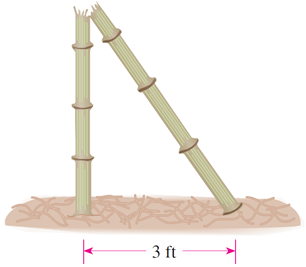
\includegraphics[scale = 0.7]{bamboo.png}
\caption{Diagram from Problem 3}
\end{figure}

\vspace{0.2cm} 
\textbf{Question 3 Solution:}\\

Consider labeling all three sides of the triangle in the diagram given. The hypotenuse is c while the other sides are a and b. We know that a, or the bottom side, is 3 ft long.
\begin{center}

\includegraphics[scale = 0.2]{A1-3 Diagram.png}
\end{center}

From Pythagorean Theorum (PT) we know that $a^2 + b^2 = c^2$ or in this case $3^2 + b^2 = c^2$. 
We also know from the question that $b+c = 10$. Therefore, with 2 equations we can solve for the unknow values: b and c.

\vspace{-1.5em}
\begin{align*}
    \text{\space} c^2 & = \text{\space} b^2 + 9 && (1)\\[-1em]
    \text{\space} 10 & = \text{\space} b + c && (2)
\end{align*}

Rearrange the second equation $10 = b + c$ to isolate one of the variables to solve by substitution. I am isolating c to solve for b (the height).

\begin{align*}
    10 & = b + c \\
    \\[-4.5em]
    10 - b & = c && \text{(3) \space \space subtract b from all}
\end{align*}

\vspace{0.2em}
\begin{center}
    \textbf{Continue solution on next page}\\
\end{center}

\newpage

\vspace{0.2cm}
\begin{center}
    Now substitute (3) into (1) as c and solve for b:
\end{center}

\vspace{-2em}
\begin{align*}
    c^2 & = b^2 + 9 && \text{(1)} \\
    (10 - b)^2 & = b^2 + 9 && \text{(3) into (1) as c} \\
    100 -20b + b^2 & = b^2 + 9 && \text{expand square} \\
    100 - 20b & = 9 && \text{subtract} b^2 \text{from both sides} \\
    100 - 9 & = 20b && \text{subtract 9 and -20b from both sides} \\
    91 & = 20b && \text{simplify} \\
    b & = \frac{91}{20} && \text{divide 20 from both sides} \\ 
\end{align*}

\vspace{-4em}
\begin{center}
    $\therefore$ the height of the vertical bamboo shoot (break) is $\boxed{\frac{91}{20} \text{ft}}$ or 4.55 ft
\end{center}

%proof/check
\vspace{1em}
\begin{proof}
    \textbf{Check answer by solving for c with (2) and then confirming result with (1)}
    \begin{align*}
        10 - b & = c && \text{From (3)} \\
        c & = 10 - 4.55 && \text{substitute b for 4.55} \\
        c & = 5.45
    \end{align*}

    \begin{center}
        Now substitute b and c values into (1) to prove the equivalent values
    \end{center}

    \vspace{-1em}
    \begin{align*}
        c^2 & = b^2 + 9 && \text{From (1)}\\
        {(5.45)}^2 & = {(4.55)}^2 + 9 && \text{substitute the values of b and c} \\
        29.7025 & = 20.7025 + 9 && \text{expand and simplify} \\
        29.7025 & = 29.7025 \\
        \text{LHS} & = \text{RHS} && \qedhere
    \end{align*}
        
\end{proof}

\newpage

%% PROBLEM 4
\item \textbf{Define} (rewrite) $f(x) = |x^3 - x|$ as a piecewise function not including any expressions involving absolute value.


\newpage

%% PROBLEM 5
\item \textbf{Determine} the inverse of the function $g(x)=\dfrac{-2}{x-1}+4$. \textbf{Prove} that $g$ and $g^{-1}$ satisfy the expression $g(g^{-1}(x))=x$.

\newpage

\end{enumerate}
\end{document} 
